\documentclass[twocolumn]{rbef}

% $if(highlighting-macros)$
% $highlighting-macros$
% $endif$

\usepackage{lipsum}

\usepackage{bbm}
\usepackage{subfig}
\usepackage{pdfpages} % Para incluir a capa.

\hypersetup{%
    pdfborder = {0 0 0}
}

\newcommand{\1}{\mathbbm{1}}
\newcommand{\s}{\mathcal{S}}
\newcommand{\T}{\mathcal{T}}
\newcommand{\A}{\mathcal{A}}
\newcommand{\ket}{\rangle}
\newcommand{\bra}{\langle}

\newtheorem{defi}{Definição}
\newtheorem{theorem}{Teorema}
\newtheorem{acknowledgement}[theorem]{Acknowledgement}
\newtheorem{algorithm}[theorem]{Algorithm}
\newtheorem{axiom}[theorem]{Axiom}
\newtheorem{claim}[theorem]{Claim}
\newtheorem{conclusion}[theorem]{Conclusion}
\newtheorem{condition}[theorem]{Condition}
\newtheorem{conjecture}[theorem]{Conjecture}
\newtheorem{corollary}[theorem]{Corollary}
\newtheorem{criterion}[theorem]{Criterion}
\newtheorem{definition}[theorem]{Definition}
\newtheorem{example}[theorem]{Example}
\newtheorem{exercise}[theorem]{Exercise}
\newtheorem{lemma}[theorem]{Lemma}
\newtheorem{notation}[theorem]{Notation}
\newtheorem{problem}[theorem]{Problem}
\newtheorem{proposition}[theorem]{Proposition}
\newtheorem{remark}[theorem]{Remark}
\newtheorem{solution}[theorem]{Solution}
\newtheorem{summary}[theorem]{Summary}
\newenvironment{proof}[1][Proof]{\noindent\textbf{#1.} }{\ \rule{0.5em}{0.5em}}

\titulocabecalho{Utilizando a Regressão Logística para Classificação de Churn em um Ambiente de Startup}
\autorcabecalho{Antonio C. da Silva Júnior}

\numeracao{01}
\volume{01}
\numero{01}
\ano{2019}
\doi{http://dsbd.leg.ufpr.br/tcc}
% \tipodeartigo{TCC DSBD}
\tipodeartigo{Especialização em Data Science \& Big Data}
% \addtocounter{page}{566} %% \setcounter produces extra white page!!! use ===\addtocounter===

\author[1]{Antonio C. da Silva Júnior}

\affil[1]{Campus Santos, Universidade Paulista
  Av. Conselheiro Nébias 766, Boqueirão, 11045-002, Santos, SP,
  Brasil\thanks{\href{emailto:juniorssz@gmail.com}{juniorssz@gmail.com}}
}
% https://www.unip.br/presencial/universidade/campi/santos.aspx
% \author[2]{Alan C. Santos}

% \affil[2]{Instituto de Física, Universidade Federal Fluminense
%   Av. General Milton Tavares de Sousa s/n, Gragoatá, 24410-346, Niterói,
%   RJ, Brasil\thanks{\href{emailto:alancs@if.uff.br}{alancs@if.uff.br}}
% }

\titulo{Utilizando a Regressão Logística para Classificação de Churn em um Ambiente de Startup}

\subtitulo{Using Logistic Regression for Churn Classification in a Startup Environment}

% -----------------------------------------------------------------------

\begin{document}

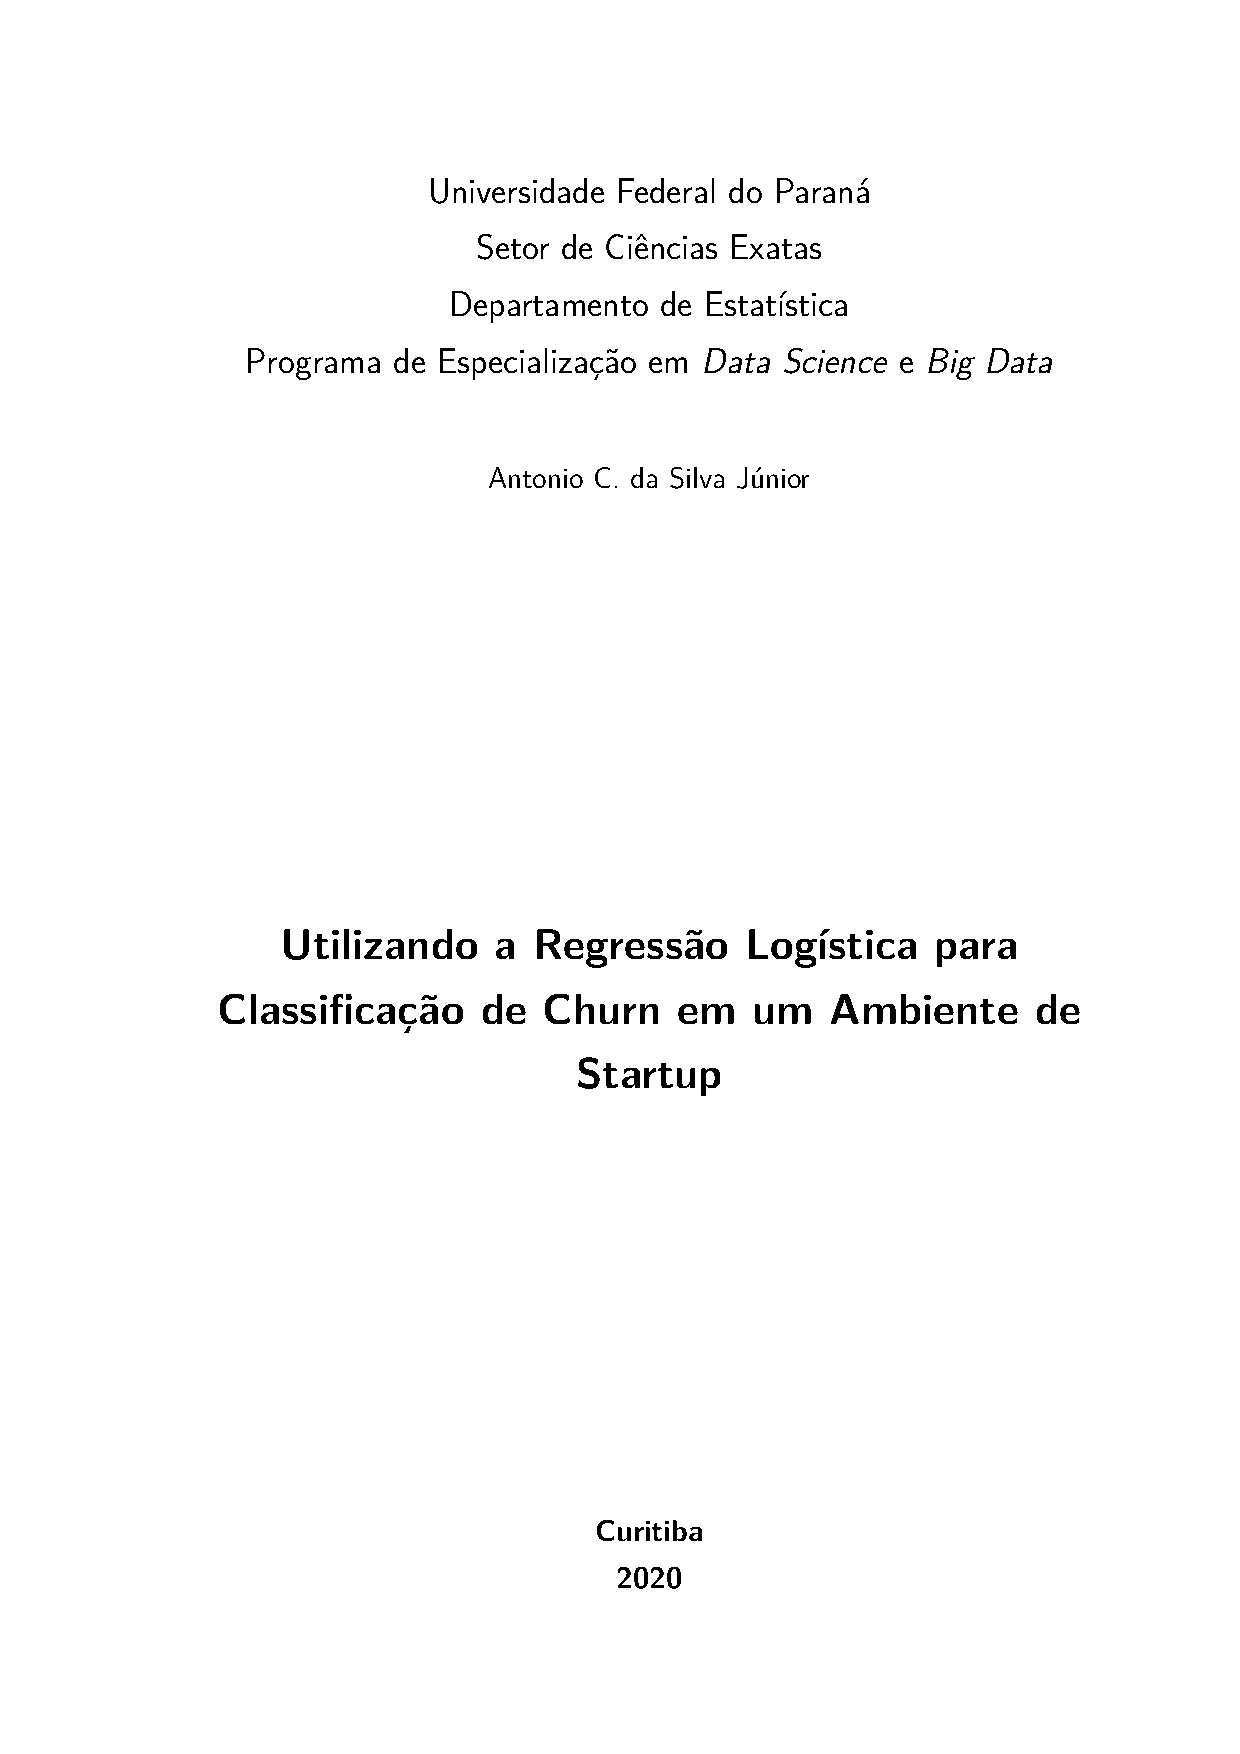
\includepdf[pages=-]{cover.pdf} % Incluí a capa

\begin{primeirapagina}

  % \begin{center}
  %   \vspace{-12pt} \small{Recebido em xxx. Aceito em xxx}
  % \end{center}

  \begin{abstract}
    Um desenvolvimento didático para determinar a solução da
    equação de movimento para uma partícula carregada imersa em
    uma região na presença de campos elétrico e magnéticos
    estáticos genéricos é proposto. Nossa proposta tem como
    alicerce a vantagem de, utilizando as propriedades da
    transformada de Laplace, podermos mapear um sistema de
    equações diferenciais não-homogêneas de segunda ordem no
    problema simples de encontrar as soluções de um sistema linear
    de equações. A partir da solução mais geral possível para o
    sistema, estudamos alguns casos particulares e recuperamos de
    forma simples alguns resultados já existentes na literatura. A
    fim de motivar nosso estudo, partimos do Teorema de Ehrenfest
    e discutimos como os resultados obtidos para o caso clássico
    podem ser interpretados na sua versão quântica.
    \palavraschave{movimento de cargas, campos elétrico e
      magnético, trajetória, análogo quântico}

  \end{abstract}

  \begin{otherlanguage}{english}


    \begin{abstract}
      A didactic development to determinate the solution of the
      motion equations for a charged particle under influence of
      electric and magnetic static fields is proposed. Our proposed
      uses the advantages and proprieties of the Laplace’s
      transformation, to map a system of N non-homogeneous
      differential equations of second order in a system composed by
      N linear equations. From the solution more general for
      dynamics of the system, we study some particular cases to
      recover, of a simple way, the results present in the
      literature. In order to give a motivation to our study, we use
      the Ehrenfest’s theorem and we discuss as the classical
      results can be interpreted in its quantum version.
      \keywords{Charge moving, electric and magnetic fields,
        trajectory, quantum analogue}

    \end{abstract}
  \end{otherlanguage}

\end{primeirapagina}
\saythanks

$body$

\bibliographystyle{unsrt}
\bibliography{referencias}

\end{document}